%-- Add sections and your outline will be created automatically --%
\section{Tephra settling}

% Frame starts a new slide
\begin{frame}
  \frametitle{Tephra settling}
  \begin{itemize}
    \item Fluidity is used to replicate a laboratory experiment of tephra (fine volcanic ash
particles) settling through a tank of water (Carey, 1997).\newline
    \item Small tephra particles can settle either individually, or collectively as a cloud of particles (a plume).\newline
    \item Plumes are generated when the bulk density of the tephra-water mixture becomes large enough, yielding settling velocities much greater than those expected of single particles (which settle at a velocity given by Stokes law).
  \end{itemize}
\end{frame}

\begin{frame}
  \frametitle{Tephra settling - Simulation setup}
  \begin{itemize}
    \item The simulation uses a 0.3 x 0.7 metre domain, replicating the cross-section of the water tank used in the experiments.\newline
    \item No normal flow boundary conditions are weakly imposed along with a zero velocity initial condition, and the initial volume fraction of the particle phase is set to $1.0 \times 10^{-7}$.\newline
    \item The influx of particles from the air above is simulated using a \texttt{flux} boundary condition at the top of the domain. This allows tephra to flux in at a rate of $0.472\ \mathrm{gm^{-2}s^{-1}}$.
  \end{itemize}
\end{frame}

\begin{frame}
  \frametitle{Tephra settling - Numerical results (1)}
\begin{figure}[H]
        \centering
                
\includegraphics[scale=0.2]{tephra_settling/tephra_fine_1.png}\hspace{0.1cm}
                
\includegraphics[scale=0.2]{tephra_settling/tephra_fine_2.png}\hspace{0.1cm}
                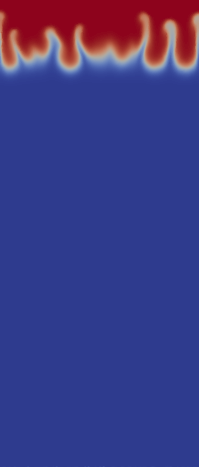
\includegraphics[scale=0.2]{tephra_settling/tephra_fine_3.png}\hspace{0.1cm}
                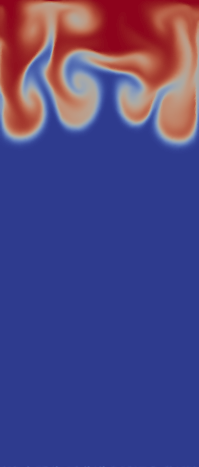
\includegraphics[scale=0.2]{tephra_settling/tephra_fine_4.png}\hspace{0.1cm}
                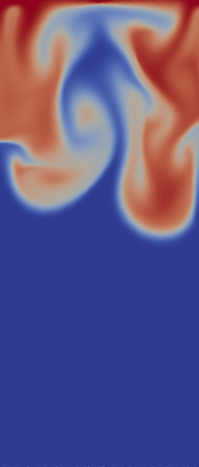
\includegraphics[scale=0.2]{tephra_settling/tephra_fine_5.png}
   \label{fig:tephra_adaptive}
   \caption{Simulation visualisations at $t = 10, 30, 50, 80$ and $110$ seconds. Tephra particles initially settle individually, but as more tephra fluxes in, the layer eventually becomes unstable and plumes begin to form.}
\end{figure}
\end{frame}

\begin{frame}
  \frametitle{Tephra settling - Numerical results (2)}
\begin{figure}[H]
        \centering
                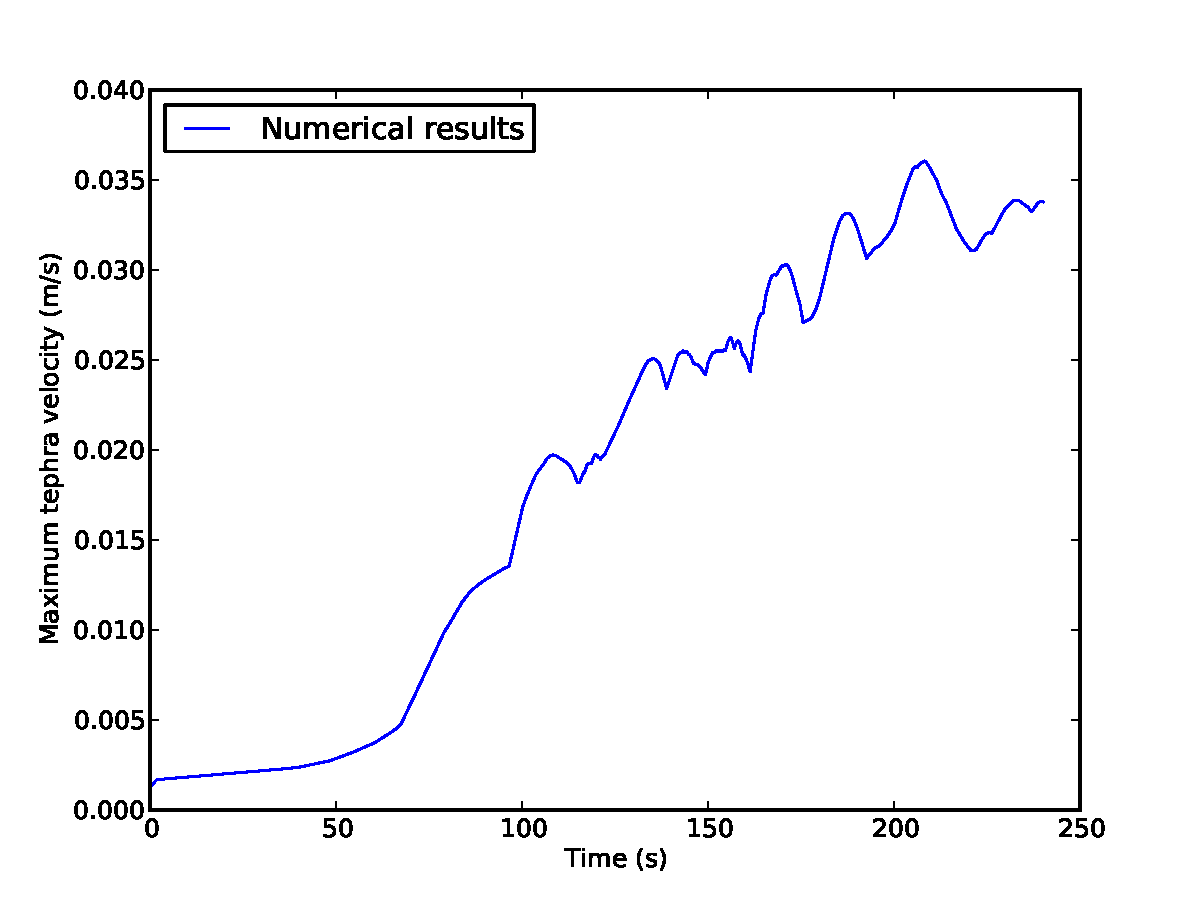
\includegraphics[scale=0.27]{tephra_settling/tephra_velocity.pdf}
   \label{fig:tephra_velocity}
   \caption{Plot of the maximum tephra phase velocity against time. Tephra particles initially settle at approximately $0.0017\ \mathrm{ms^{-1}}$, as predicted by Stokes' law. Plumes begin to form after approximately 30 seconds, resulting in settling velocities over 10 times greater than that of an individual particle.}
\end{figure}
\end{frame}

\begin{frame}
  \frametitle{Tephra settling - Exercises}
 \begin{itemize}
    \item Decrease the characteristic element size to better resolve the plume behaviour.\newline
    \item Alter the particle size to observe its effect on plume formation.\newline
    \item Add a second particle phase (with a different particle size).
 \end{itemize}
\end{frame}


